\textbf{Входные параметры:}
 
 Fitness --- массив пригодностей (можно подавать не массив пригодностей, а массив значений целевой функции, но только для задач безусловной оптимизации);
  
 VMHL\_N --- размер массива пригодностей.

\textbf{Возвращаемое значение:} 

Номер выбранной пригодности, а, соответственно, номер индивида популяции.

 \textbf{Принцип работы:}

\begin{figure} [h]
  \center
  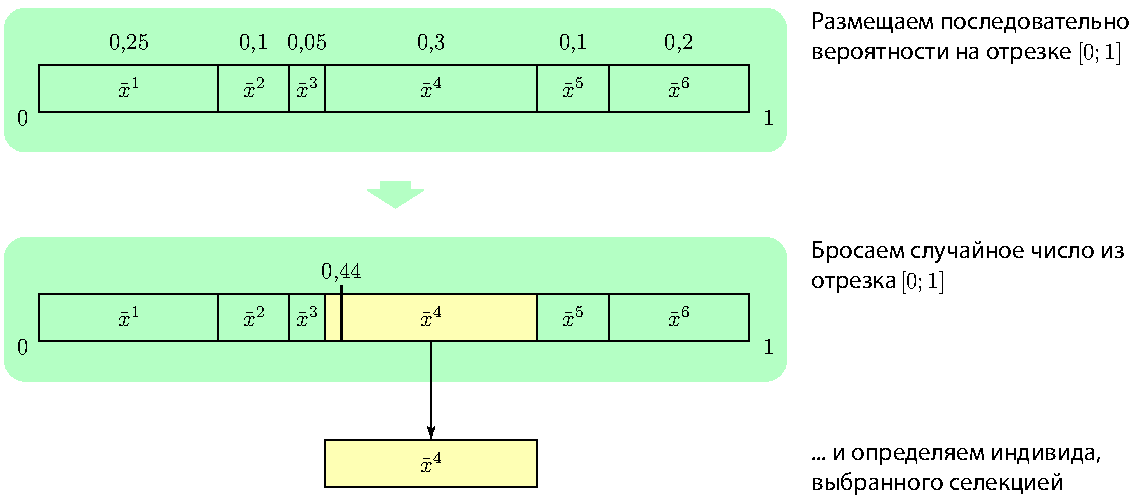
\includegraphics [scale=0.8] {MHL_ProportionalSelection_Sheme}
  \caption{Механизм работы пропорциональной селекции} 
  \label{img:MHL_ProportionalSelection_Sheme}  
\end{figure}

\textbf{Примечание:}

 Использовать реализацию оператора ГА в виде этой функции нецелесообразно ввиду того, что при каждом запуске создается дополнительный массив.  Данная функция аналогична по действию (результат действия аналогичен):
 
 \begin{enumerate}
\item Связке функций MHL\_MakeVectorOfProbabilityForProportionalSelectionV2 и MHL\_ProportionalSelectionV2;
\item Функции MHL\_ProportionalSelectionV3.
 \end{enumerate}
 
Различия по временным затратам на выполнение. У этой реализации самое большое время выполнения.
  
\textbf{Примечание:}

 Под массивом пригодностей понимается специально преобразованный массив значений целевой функции. Процесс подробно описан в стандарте генетического алгоритма. Смотреть здесь. Но это если Вы используете в алгоритмах оптимизации подобных генетическому. а так, если будете использовать, то учитывайте, что массив пригодностей --- это массив вещественных чисел из отрезка $[0;1]$.
